\documentclass[a4paper]{article}
\usepackage[english]{babel}
\usepackage[english]{isodate}  		% english date format
\usepackage{textcomp, gensymb}      % to avoid some warnings
\usepackage{graphicx}				% image management
\usepackage{amsfonts}               % math fonts
\usepackage{booktabs}				% improve tables
\usepackage{amsmath}				% another math. pack.
% \usepackage{mathtools}				% underline under eq.
% \usepackage{stmaryrd} 				% for '\llbracket' and '\rrbracket'
% \usepackage{amsthm}					% better theorems
\usepackage{enumitem}				% list management
\usepackage{pifont}					% 'cute' bullet points
% \usepackage{cancel}					% cancel math expressions
\usepackage{caption}				% custom caption
\usepackage[]{mdframed}				% text box
\usepackage{multirow}				% table rows
\usepackage{gensymb}				% degree symbol
\usepackage[x11names]{xcolor}		% RGB colors pack.
\usepackage{tcolorbox}				% color box text
\usepackage{eurosym}

% draw a frame around given text
\newcommand{\framedtext}[1]{%
	\par%
	\noindent\fbox{%
		\parbox{\dimexpr\linewidth-2\fboxsep-2\fboxrule}{#1}%
	}%
}

% hypertext
\usepackage{xcolor}
\usepackage[linkcolor=black, citecolor=blue, urlcolor=cyan]{hyperref}
\hypersetup{
	colorlinks=true
}

% sorry, I don't use a US keyboard
\newcommand{\dquotes}[1]{``#1''}
\newcommand{\longline}{\noindent\rule{\textwidth}{0.4pt}}

\begin{document}
    \author{VR443470 - Valentini Andrea}
    \title{University of Verona \\
    \:\\
    Programming FPGA on cloud - Guide}
    \date{Last Update: \today}

    \maketitle

    \newpage

    \tableofcontents

    \newpage

    \section{Amazon}

    \subsection{Introduction to AWS}

    This guide is designed to help some developers, and not, to explore the cloud technologies to learn how to program an FPGA (on cloud).

    \longline
    
    \subsubsection{Register a new account}

    From this site you can register on the AWS platform: \url{https://aws.amazon.com/}. You can create an account choosing two possibility plans:
    \begin{itemize}
        \item Personal account, with some limitations (see more: \href{https://aws.amazon.com/free/?all-free-tier.sort-by=item.additionalFields.SortRank&all-free-tier.sort-order=asc&awsf.Free%20Tier%20Types=*all&awsf.Free%20Tier%20Categories=*all}{here});

        \item Business account, but attention because you need to register a payment card (see more: \href{https://aws.amazon.com/premiumsupport/plans/}{here}).
    \end{itemize}
    Although, there is an opportunity to students, and anyone else has an institutional e-mail, to register on the AWS Educate platform\footnote{FAQ: \url{https://www.awseducate.com/registration/s/faqs?language=en_US}}: \url{https://aws.amazon.com/education/awseducate/}. This plan allows you to access to AWS Educate lab, which provides access to the AWS Console to enable practical application of concepts without the need for credits (in summary, more resources without having to pay).\newline
    Unfortunately, Education Plan doesn’t give you the \dquotes{freedom} to do whatever you want because use AWS Console only meanwhile a learn course (sandbox).
    This choice is still valid because you can use the various tutorials to create guides (like this) or understand how-to-use EC2 F1.
    \begin{figure}[!htp]
        \centering
        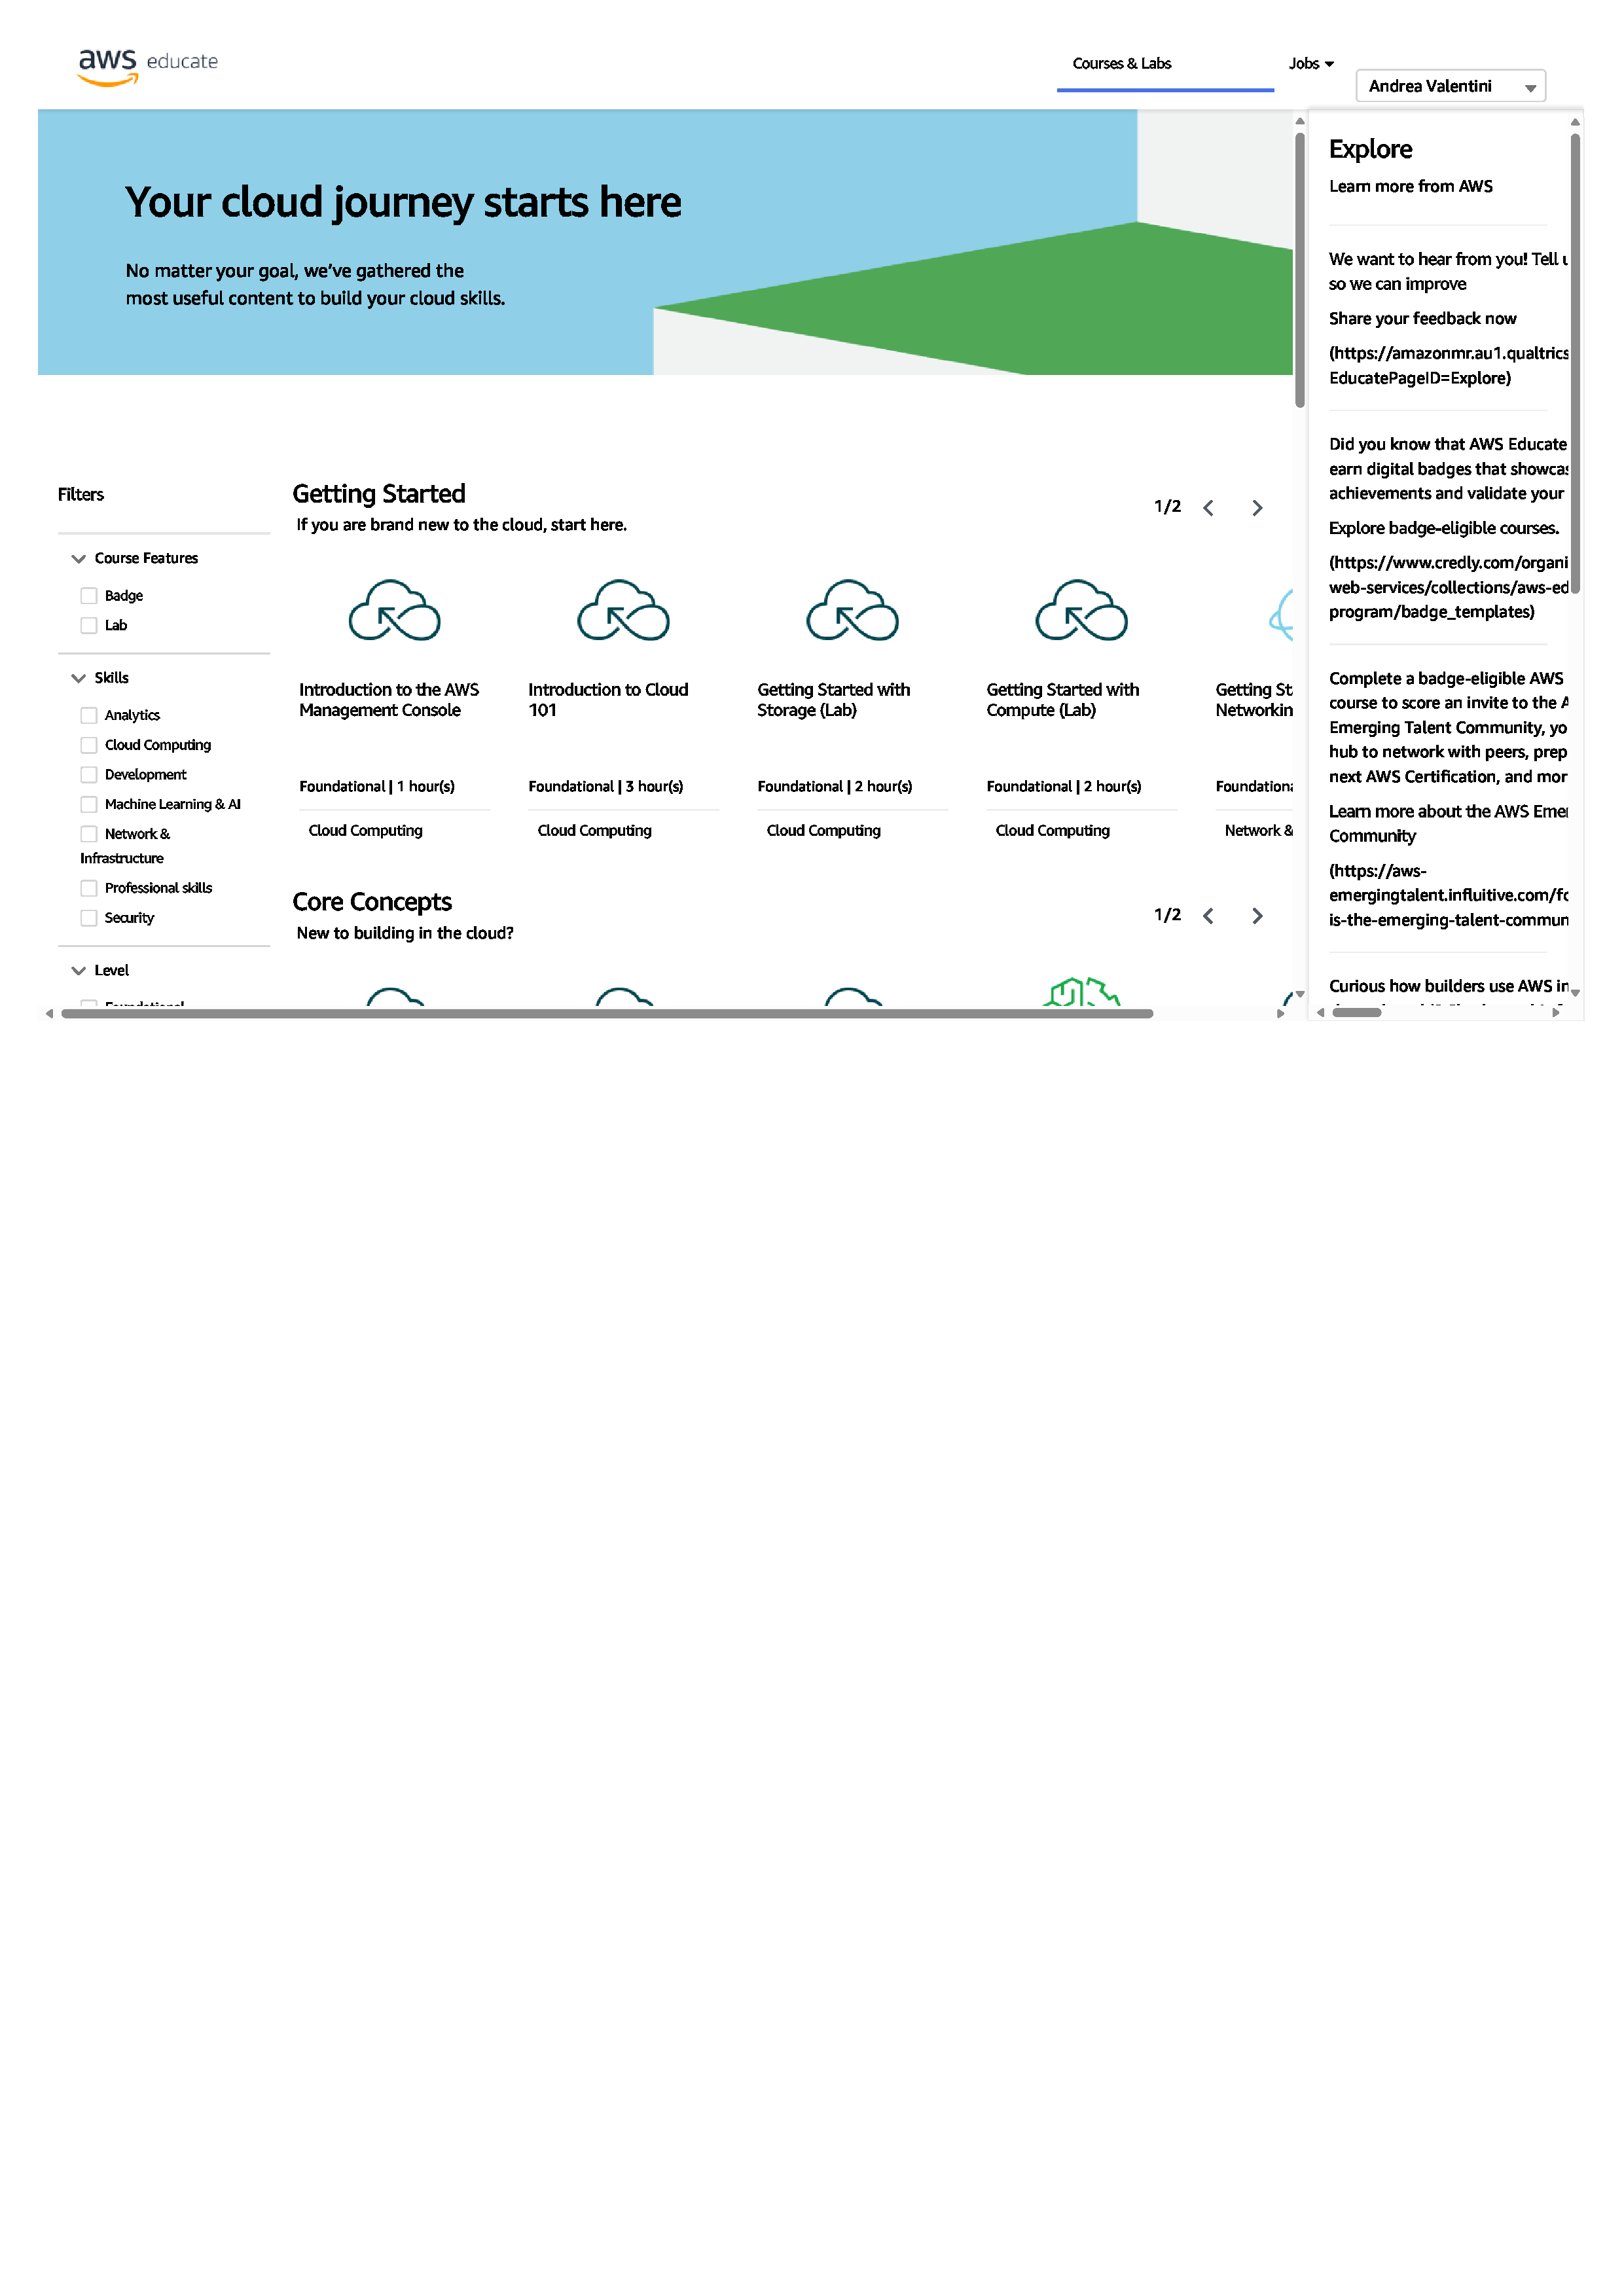
\includegraphics[width=\textwidth]{img/AWS Educate Dashboard.pdf}
        \caption{AWS Educate Dashboard.}
    \end{figure}\newpage

    \noindent
    If you've chosen to use a personal/business plan, once inserted a pay card number, and confirmed it with a 1\$ fee you should have this screen:
    \begin{figure}[!htp]
        \centering
        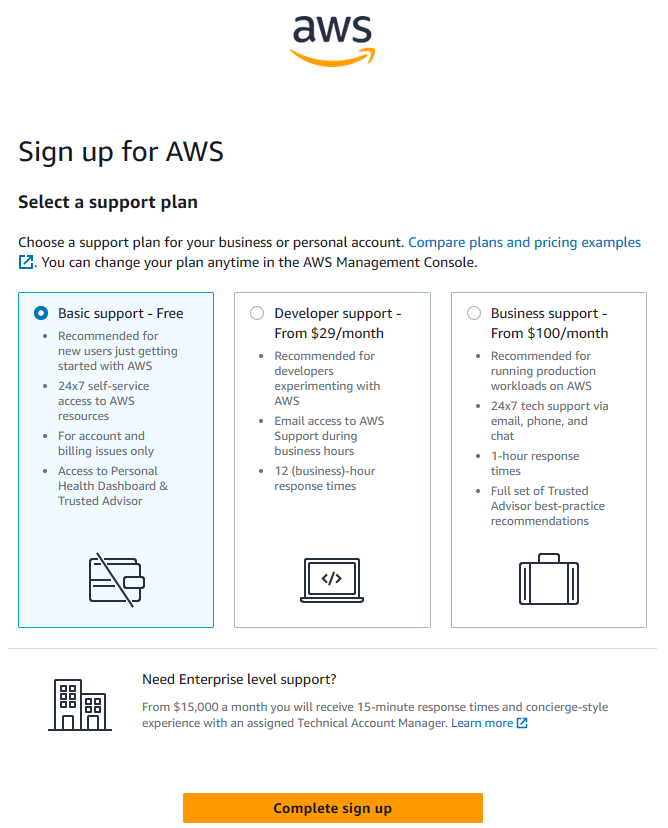
\includegraphics[width=\textwidth]{img/sing-up.png}
    \end{figure}

    \noindent
    On this figure, you can also see the various plans offered. To compare plans and pricing examples, you can visit this page: \href{https://aws.amazon.com/premiumsupport/plans/}{link}.\newline

    \noindent
    Anyway, choosing a Free plan will automatic start an AWS Free Tier (\href{https://aws.amazon.com/free/terms/}{terms}). The 12 Month Free Tier is only available to new AWS customers, and is available for 12 months following your AWS sign-up date.

    If you have not used the AWS resources provided under an Offer during the previous 3 months, we may reclaim those AWS resources after giving you 30 days' notice. Even if your AWS resources are reclaimed, you may continue to participate in Offers using new AWS resources.

    \newpage

    \subsubsection{Getting Started}

    The first thing to do to understand how AWS works is read the Getting Started guide: \url{https://aws.amazon.com/getting-started/}. In this site, you can find some useful guides that explain cloud functions and others Amazon products.\newline

    \noindent
    After that, AWS shows you a sea of tutorials such as \dquotes{Build a Serverless Web Application}, \dquotes{Deploy a Web Application on Amazon EC2}, etc. Here's the link: \href{https://aws.amazon.com/getting-started/hands-on/?pg=gs&sec=lyfa&getting-started-all.sort-by=item.additionalFields.content-latest-publish-date&getting-started-all.sort-order=desc&awsf.getting-started-category=*all&awsf.getting-started-content-type=*all}{Hands-on Tutorials}.\newline

    \noindent
    If you chosen a Business (or free) account plan, this is your dashboard:
    \begin{figure}[!htp]
        \centering
        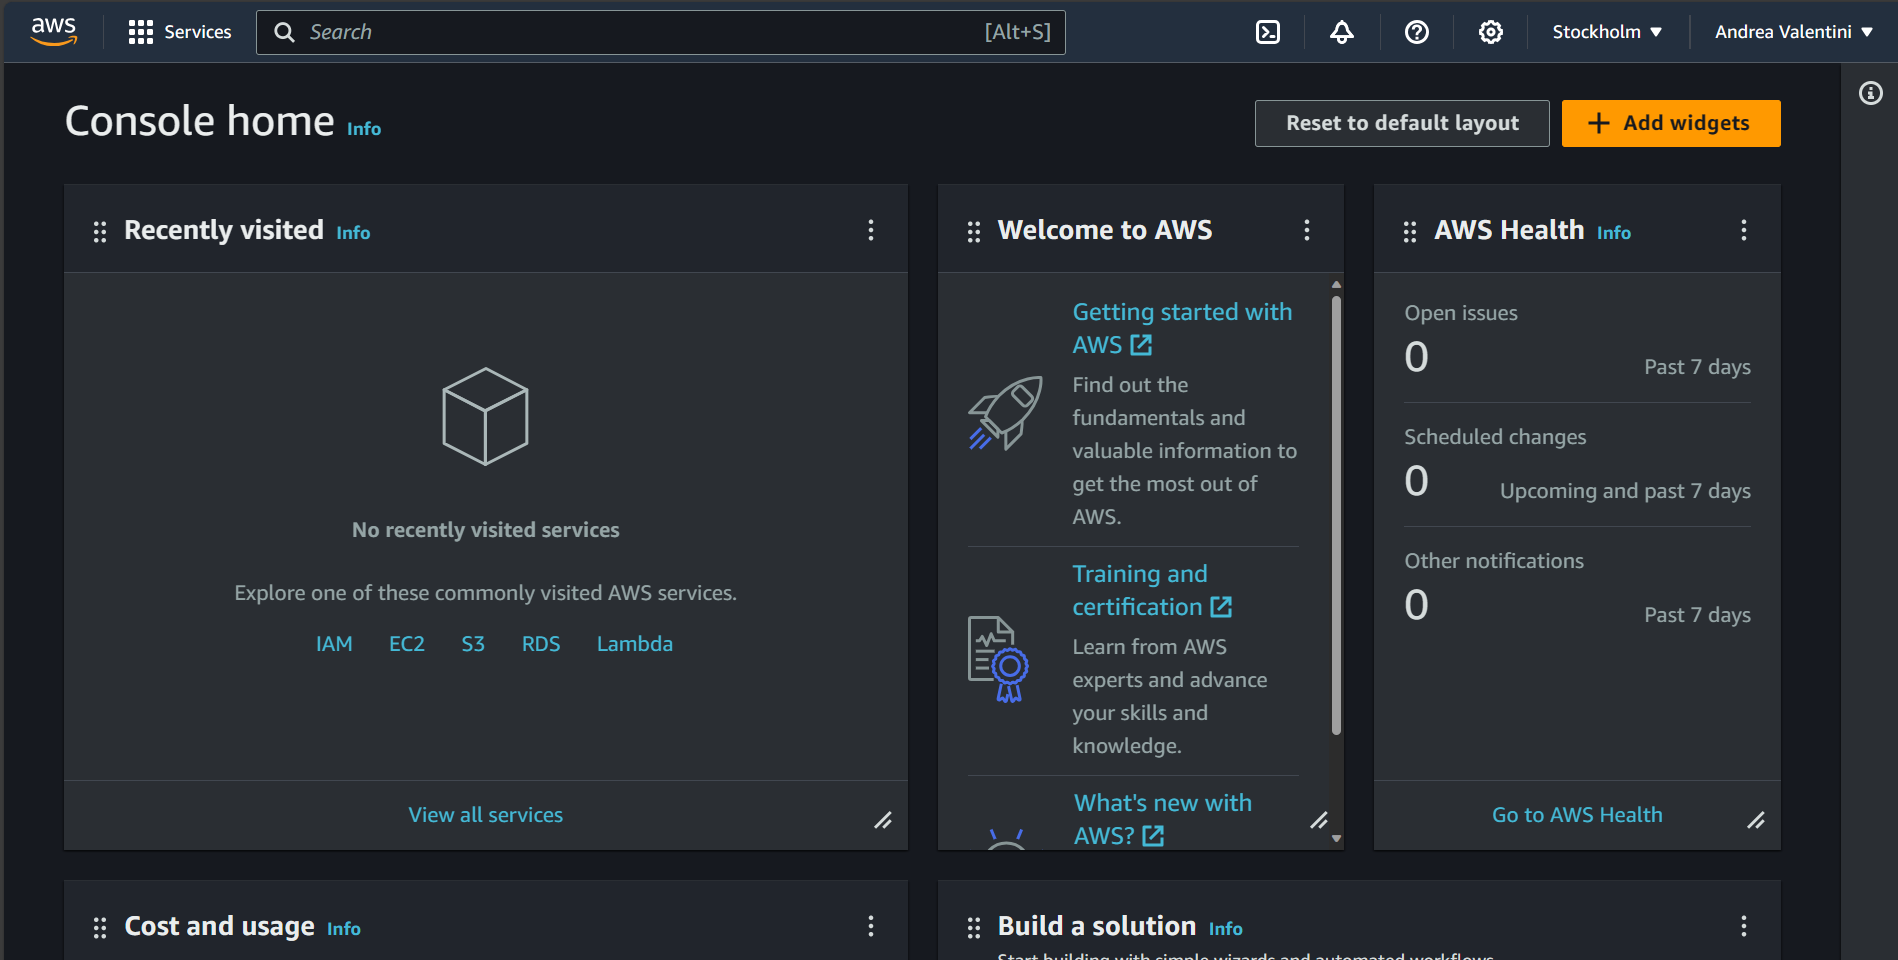
\includegraphics[width=\textwidth]{img/business-free_dashboard.png}
        \caption{AWS Business/Free Dashboard.}
    \end{figure}

    \noindent
    On the left side you can see all resources created and recently visited; at the top you can see all hypertext link that can help you to start.\newpage

    \subsection{Amazon EC2 F1 Instances}

    \subsubsection{Description}

    Amazon EC2 F1 instances use FPGAs to enable delivery of custom hardware accelerations. With F1 instances you can:
    \begin{itemize}
        \item Develop
        \item Simulate
        \item Debug
        \item Compile
    \end{itemize}
    hardware acceleration code, including an FPGA Developer AMI (see \ref{sec: FPGA Developer AMI} cap.). Furthermore, EC2 supporting hardware level development on the cloud.\newline

    \noindent
    F1 instances provide diverse development environments: from low-level hardware developers to software developers who are more comfortable with C/C++ and openCL environments (see more on \ref{sec: development kit} par.).\newline

    \noindent
    Once your FPGA design is complete, you can register it as an Amazon FPGA Image (AFI), and deploy it to your F1 instance in just a few clicks. You can reuse your AFIs as many times as you like, and across as many F1 instances as you like. There is no software charge for the development tools when using the FPGA developer AMI and you can program the FPGAs on your F1 instance as many times as you like with no additional fees.\newline

    \noindent
    Instances Features:
    \begin{itemize}
        \item High frequency Intel Xeon Scalable Processors (Broadwell E5-2686 v4)
        \item NVMe SSD Storage
        \item Support for Enhanced Networking
    \end{itemize}
    FPGA Features:
    \begin{itemize}
        \item Xilinx Virtex UltraScale+ VU9P FPGAs
        \item 64 GiB of ECC-protected memory on 4x DDR4
        \item Dedicated PCI-Express x16 interface
        \item Approximately 2.5 million logic elements
        \item Approximately 6,800 Digital Signal Processing (DSP) engines
        \item FPGA Developer AMI (see \ref{sec: FPGA Developer AMI})
    \end{itemize}\newpage

    \begin{table}[!htp]
        \centering
        \begin{tabular}{@{} l p{4em} p{4em} p{4em} p{4em} p{6em} @{}}
            \toprule
            \textbf{Instance} & \textbf{FPGAs} & \textbf{vCPU} & \textbf{Memory (GiB)} & \textbf{Instance Storage (GB)} & \textbf{Networking Performance (Gbps)***} \\
            \midrule
            \texttt{f1.2xlarge}     & 1 & 8 & 122 & $1 \times 470$ & Up to 10 \\
            \texttt{f1.4xlarge}     & 2 & 16 & 244 & $1 \times 940$ & Up to 10 \\
            \texttt{f1.16xlarge}    & 8 & 64 & 976 & $4 \times 940$ & 25 \\
            \bottomrule
        \end{tabular}
        \caption{The specifications of each type of \emph{EC2 F1 Instances}.}
        \label{tab: the specifications of each type of EC2 F1 Instances}
    \end{table}
    For \texttt{f1.16xlarge} instances, the dedicated PCI-e fabric lets the FPGAs share the same memory space and communicate with each other across the fabric at up to 12 Gbps in each direction.\newline

    \noindent
    All instances have the following specs:
    \begin{itemize}
        \item 2.3 GHz (base) and 2.7 GHz (turbo) Intel Xeon E5-2686 v4 Processor

        \item \href{https://aws.amazon.com/ec2/instance-types/#Intel}{Intel AVX*, Intel AVX2*, Intel Turbo}

        \item \href{https://aws.amazon.com/ec2/instance-types/#EBS}{EBS Optimized}

        \item \href{https://aws.amazon.com/ec2/details/#enhanced-networking}{Enhanced Networking*}
    \end{itemize}
    * AVX and AVX2 are only available on instances launched with HVM AMIs.\newline

    \noindent
    *** Instances marked with "Up to" Network Bandwidth have a baseline bandwidth and can use a network I/O credit mechanism to burst beyond their baseline bandwidth on a best effort basis. For more information, see \href{https://docs.aws.amazon.com/AWSEC2/latest/UserGuide/ec2-instance-network-bandwidth.html}{instance network bandwidth}.\newpage

    \subsubsection{Amazon EC2 Pricing}
    
    The following table is a summary of the prices available. The costs depend on which nation you choose.

    \begin{table}[!htp]
        \centering
        \begin{tabular}{@{} p{5em} p{7em} p{10em} p{10em} @{}}
            \toprule
            \begin{center}
                \textbf{Name}
            \end{center}
            & \begin{center}
                \vspace{-1.5em}
                \textbf{On-Demand Price/hr}
                \vspace{-1em}
            \end{center} 
            & \begin{center}
                \vspace{-1.5em}
                \textbf{1-yr Reserved Instance Effective Hourly}
                \vspace{-1em}
            \end{center}
            & \begin{center}
                \vspace{-1.5em}
                \textbf{3-yr Reserved Instance Effective Hourly}
                \vspace{-1em}
            \end{center} \\
            \midrule
            %
            \begin{center}
                \vspace{-1.9em}
                \texttt{f1.2xlarge}
            \end{center} &
            \begin{center}
                \vspace{-1.5em}
                \$1.65
            \end{center} & 
            \begin{center}
                \vspace{-1.5em}
                \$1.06
            \end{center} & 
            \begin{center}
                \vspace{-1.5em}
                \$0.76
            \end{center} \\
            %
            \begin{center}
                \vspace{-2.5em}
                \texttt{f1.4xlarge}
            \end{center} &
            \begin{center}
                \vspace{-2em}
                \$3.30
            \end{center} & 
            \begin{center}
                \vspace{-2em}
                \$2.12
            \end{center} & 
            \begin{center}
                \vspace{-2em}
                \$1.52
            \end{center} \\
            %
            \begin{center}
                \vspace{-2.5em}
                \texttt{f1.16xlarge}
                \vspace{-2em}
            \end{center} &
            \begin{center}
                \vspace{-2em}
                \$13.20
                \vspace{-2em}
            \end{center} & 
            \begin{center}
                \vspace{-2em}
                \$8.50
                \vspace{-2em}
            \end{center} & 
            \begin{center}
                \vspace{-2em}
                \$6.10
                \vspace{-2em}
            \end{center} \\
            \bottomrule
        \end{tabular}
        \caption{Prices shown are for Linux/Unix in the US East (Northern Virginia) AWS Region and rounded to the nearest cent. Prices for 1-year and 3-year reserved instances are for "Partial Upfront" payment options.}
        \label{tab: how much ec2 f1 costs}
    \end{table}

    \noindent
    You can visit the price page for more details: \href{https://aws.amazon.com/ec2/pricing/}{click here}. Although Amazon says you can try EC2 F1 for free, this is untrue. Amazon allows you to use (for 750 hours) a virtual instance (a virtual resource) to give you a taste. Instead, Amazon EC2 F1 are dedicated instances (FPGA).\newline

    \noindent
    At least you can estimate the costs with the \href{https://calculator.aws/#/createCalculator/ec2-enhancement}{AWS Pricing Calculator}.

    \longline

    \subsubsection{Development Kit}\label{sec: development kit}

    Once you created an AWS account, you \textbf{must} downloading the AWS FPGA Development Kit by this official repository: \url{https://github.com/aws/aws-fpga}. It includes all documentation (\href{https://github.com/aws/aws-fpga#documentation-overview}{shortcut url}) on:
    \begin{itemize}
        \item F1
        \item Internal FPGA interfaces
        \item Compiler scripts for generating Amazon FPGA Images (AFIs)
    \end{itemize}
    
    \noindent
    AWS FPGAs support multiple development environments to serve both hardware and software developers:
    \begin{itemize}
        \item The FPGA Hardware Development Kit (HDK, \href{https://github.com/aws/aws-fpga#hardware-development-kit-hdk}{shortcut url}) provides fully custom hardware development;

        \item The FPGA Software Development Kit (SDK, \href{https://github.com/aws/aws-fpga#runtime-tools-sdk}{shortcut url}) environment allows developing accelerations using C/C++/OpenCL code with no hardware knowledge needed.
    \end{itemize}
    Again, this kit is \textbf{essential to develop fast FPGA for the EC2 F1 instances}.\newpage

    \subsubsection{FPGA Developer AMI}\label{sec: FPGA Developer AMI}

    The FPGA Developer AMI is an Amazon Linux 2 based AMI provided by Amazon Web Services. The AMI is pre-built with FPGA development tools required to develop and use custom FPGAs for hardware acceleration. The FPGA Developer AMI includes Xilinx tools for simulating your FPGA design, compiling code and building your AFI (Amazon FPGA Image).\newline

    \noindent
    The FPGA Developer AMI includes Xilinx Vivado\footnote{Xilinx Vivado is a software suite produced by AMD (previously Xilinx) for synthesis and analysis of hardware description language (HDL) designs, superseding Xilinx ISE with additional features for system on a chip development and high-level synthesis. \href{https://en.wikipedia.org/wiki/Vivado}{Source}.} at no additional software charge as well as a prepackaged tool development environment with scripts and tools for simulating your FPGA design and building and registering your AFI.\newline

    \noindent
    As mentioned above, developers can deploy the FPGA Developer AMI on an Amazon EC2 instance and quickly provision the resources they need to write and debug FPGA designs in the cloud. The FPGA Developer AMI is provided at no additional charge to Amazon EC2 users.\newline

    \noindent
    Typical Total Price (updated on 17th October 2023): \$0.796/hr.\newline

    \noindent
    See more: \href{https://aws.amazon.com/marketplace/pp/prodview-iehshpgi7hcjg}{AWS marketplace}.\newpage
    
    \subsubsection{Q\&A}
    
    The following questions and answers can be found on the original site, but they're brought here for convenience (\href{https://aws.amazon.com/ec2/faqs/?nc1=h_ls#Instance_types}{source}).

    \begin{table}[!htp]
        \centering
        \begin{tabular}{@{} p{30em} c @{}}
            \toprule
            \textbf{Questions} & \textbf{Page} \\
            \midrule
            What is Amazon EC2 F1? & \hyperlink{What is Amazon EC2 F1?}{\hypergetpageref{What is Amazon EC2 F1?}} \\ [.5em]
            %
            What are FPGAs and why do I need them? & \hyperlink{What are FPGAs and why do I need them?}{\hypergetpageref{What are FPGAs and why do I need them?}} \\ [.5em]
            %
            How does F1 compare with traditional FPGA solutions? & \hyperlink{How does F1 compare with traditional FPGA solutions?}{\hypergetpageref{How does F1 compare with traditional FPGA solutions?}} \\ [.5em]
            %
            What is an Amazon FPGA Image (AFI)? & \hyperlink{What is an Amazon FPGA Image (AFI)?}{\hypergetpageref{What is an Amazon FPGA Image (AFI)?}} \\ [.5em]
            %
            How do I list my hardware acceleration on the AWS Marketplace? & \hyperlink{How do I list my hardware acceleration on the AWS Marketplace?}{\hypergetpageref{How do I list my hardware acceleration on the AWS Marketplace?}} \\ [.5em]
            %
            What is available with F1 instances? & \hyperlink{What is available with F1 instances?}{\hypergetpageref{What is available with F1 instances?}} \\ [.5em]
            %
            Do I need to be an FPGA expert to use an F1 instance? & \hyperlink{Do I need to be an FPGA expert to use an F1 instance?}{\hypergetpageref{Do I need to be an FPGA expert to use an F1 instance?}} \\ [.5em]
            %
            I'm an FPGA developer; how do I get started with F1 instances? & \hyperlink{I'm an FPGA developer; how do I get started with F1 instances?}{\hypergetpageref{I'm an FPGA developer; how do I get started with F1 instances?}} \\ [.5em]
            %
            I'm not an FPGA developer; how do I get started with F1 instances? & \hyperlink{I'm not an FPGA developer; how do I get started with F1 instances?}{\hypergetpageref{I'm not an FPGA developer; how do I get started with F1 instances?}} \\ [.5em]
            %
            Does AWS provide a developer kit? & \hyperlink{Does AWS provide a developer kit?}{\hypergetpageref{Does AWS provide a developer kit?}} \\ [.5em]
            %
            Can I use the HDK in my on-premises development environment? & \hyperlink{Can I use the HDK in my on-premises development environment?}{\hypergetpageref{Can I use the HDK in my on-premises development environment?}} \\ [.5em]
            %
            Can I add an FPGA to any EC2 instance type? & \hyperlink{Can I add an FPGA to any EC2 instance type?}{\hypergetpageref{Can I add an FPGA to any EC2 instance type?}} \\ [.5em]
            \bottomrule
        \end{tabular}
        \caption{Table of contents of Q\&A. Click on the the page number to go to the question/answer.}
    \end{table}

    \begin{itemize}
        \item[\ding{42}] 
        \label{What is Amazon EC2 F1?}
        \hypertarget{What is Amazon EC2 F1?}{\textbf{What is Amazon EC2 F1?}}
        \begin{itemize}
            \item[\ding{45}] Amazon EC2 F1 is a compute instance with programmable hardware you can use for application acceleration. The new F1 instance type provides a high performance, easy to access FPGA for developing and deploying custom hardware accelerations.
        \end{itemize}

        \item[\ding{42}]
        \label{What are FPGAs and why do I need them?}
        \hypertarget{What are FPGAs and why do I need them?}{\textbf{What are FPGAs and why do I need them?}}
        \begin{itemize}
            \item[\ding{45}] FPGAs are programmable integrated circuits that you can configure using software. By using FPGAs you can accelerate your applications up to 30x when compared with servers that use CPUs alone. And, FPGAs are reprogrammable, so you get the flexibility to update and optimize your hardware acceleration without having to redesign the hardware.
        \end{itemize}

        \item[\ding{42}] 
        \label{How does F1 compare with traditional FPGA solutions?}
        \hypertarget{How does F1 compare with traditional FPGA solutions?}{\textbf{How does F1 compare with traditional FPGA solutions?}}
        \begin{itemize}
            \item[\ding{45}] F1 is an AWS instance with programmable hardware for application acceleration. With F1, you have access to FPGA hardware in a few simple clicks, reducing the time and cost of full-cycle FPGA development and scale deployment from months or years to days. While FPGA technology has been available for decades, adoption of application acceleration has struggled to be successful in both the development of accelerators and the business model of selling custom hardware for traditional enterprises, due to time and cost in development infrastructure, hardware design, and at-scale deployment. With this offering, customers avoid the undifferentiated heavy lifting associated with developing FPGAs in on-premises data centers.
        \end{itemize}

        \item[\ding{42}]
        \label{What is an Amazon FPGA Image (AFI)?}
        \hypertarget{What is an Amazon FPGA Image (AFI)?}{\textbf{What is an Amazon FPGA Image (AFI)?}}
        \begin{itemize}
            \item[\ding{45}] The design that you create to program your FPGA is called an Amazon FPGA Image (AFI). AWS provides a service to register, manage, copy, query, and delete AFIs. After an AFI is created, it can be loaded on a running F1 instance. You can load multiple AFIs to the same F1 instance, and can switch between AFIs in runtime without reboot. This lets you quickly test and run multiple hardware accelerations in rapid sequence. You can also offer to other customers on the AWS Marketplace a combination of your FPGA acceleration and an AMI with custom software or AFI drivers.
        \end{itemize}

        \item[\ding{42}]
        \label{How do I list my hardware acceleration on the AWS Marketplace?}
        \hypertarget{How do I list my hardware acceleration on the AWS Marketplace?}{\textbf{How do I list my hardware acceleration on the AWS Marketplace?}}
        \begin{itemize}
            \item[\ding{45}] You would develop your AFI and the software drivers/tools to use this AFI. You would then package these software tools/drivers into an Amazon Machine Image (AMI) in an encrypted format. AWS manages all AFIs in the encrypted format you provide to maintain the security of your code. To sell a product in the AWS Marketplace, you or your company must sign up to be an AWS Marketplace reseller, you would then submit your AMI ID and the AFI ID(s) intended to be packaged in a single product. AWS Marketplace will take care of cloning the AMI and AFI(s) to create a product, and associate a product code to these artifacts, such that any end-user subscribing to this product code would have access to this AMI and the AFI(s).
        \end{itemize}

        \item[\ding{42}]
        \label{What is available with F1 instances?}
        \hypertarget{What is available with F1 instances?}{\textbf{What is available with F1 instances?}}
        \begin{itemize}
            \item[\ding{45}] For developers, AWS is providing a Hardware Development Kit (HDK) to help accelerate development cycles, a FPGA Developer AMI for development in the cloud, an SDK for AMIs running the F1 instance, and a set of APIs to register, manage, copy, query, and delete AFIs. Both developers and customers have access to the AWS Marketplace where AFIs can be listed and purchased for use in application accelerations.
        \end{itemize}

        \item[\ding{42}]
        \label{Do I need to be an FPGA expert to use an F1 instance?}
        \hypertarget{Do I need to be an FPGA expert to use an F1 instance?}{\textbf{Do I need to be an FPGA expert to use an F1 instance?}}
        \begin{itemize}
            \item[\ding{45}] AWS customers subscribing to an F1-optimized AMI from AWS Marketplace do not need to know anything about FPGAs to take advantage of the accelerations provided by the F1 instance and the AWS Marketplace. Simply subscribe to an F1-optimized AMI from the AWS Marketplace with an acceleration that matches the workload. The AMI contains all the software necessary for using the FPGA acceleration. Customers need only write software to the specific API for that accelerator and start using the accelerator.
        \end{itemize}

        \item[\ding{42}]
        \label{I'm an FPGA developer; how do I get started with F1 instances?}
        \hypertarget{I'm an FPGA developer; how do I get started with F1 instances?}{\textbf{I'm an FPGA developer; how do I get started with F1 instances?}}
        \begin{itemize}
            \item[\ding{45}] Developers can get started on the F1 instance by creating an AWS account and downloading the AWS Hardware Development Kit (HDK). The HDK includes documentation on F1, internal FPGA interfaces, and compiler scripts for generating AFI. Developers can start writing their FPGA code to the documented interfaces included in the HDK to create their acceleration function. Developers can launch AWS instances with the FPGA Developer AMI. This AMI includes the development tools needed to compile and simulate the FPGA code. The Developer AMI is best run on the latest C5, M5, or R4 instances. Developers should have experience in the programming languages used for creating FPGA code (i.e. Verilog or VHDL) and an understanding of the operation they wish to accelerate.
        \end{itemize}

        \item[\ding{42}]
        \label{I'm not an FPGA developer; how do I get started with F1 instances?}
        \hypertarget{I'm not an FPGA developer; how do I get started with F1 instances?}{\textbf{I'm not an FPGA developer; how do I get started with F1 instances?}}
        \begin{itemize}
            \item[\ding{45}] Customers can get started with F1 instances by selecting an accelerator from the AWS Marketplace, provided by AWS Marketplace sellers, and launching an F1 instance with that AMI. The AMI includes all of the software and APIs for that accelerator. AWS manages programming the FPGA with the AFI for that accelerator. Customers do not need any FPGA experience or knowledge to use these accelerators. They can work completely at the software API level for that accelerator.
        \end{itemize}

        \item[\ding{42}]
        \label{Does AWS provide a developer kit?}
        \hypertarget{Does AWS provide a developer kit?}{\textbf{Does AWS provide a developer kit?}}
        \begin{itemize}
            \item[\ding{45}] Yes. The Hardware Development Kit (HDK) includes simulation tools and simulation models for developers to simulate, debug, build, and register their acceleration code. The HDK includes code samples, compile scripts, debug interfaces, and many other tools you will need to develop the FPGA code for your F1 instances. You can use the HDK either in an AWS provided AMI, or in your on-premises development environment. These models and scripts are available publicly with an AWS account.
        \end{itemize}

        \item[\ding{42}]
        \label{Can I use the HDK in my on-premises development environment?}
        \hypertarget{Can I use the HDK in my on-premises development environment?}{\textbf{Can I use the HDK in my on-premises development environment?}}
        \begin{itemize}
            \item[\ding{45}] Yes. You can use the Hardware Development Kit HDK either in an AWS-provided AMI, or in your on-premises development environment.
        \end{itemize}

        \item[\ding{42}]
        \label{Can I add an FPGA to any EC2 instance type?}
        \hypertarget{Can I add an FPGA to any EC2 instance type?}{\textbf{Can I add an FPGA to any EC2 instance type?}}
        \begin{itemize}
            \item[\ding{45}] No. F1 instances comes in two instance sizes: f1.2xlarge, f1.4xlarge, and f1.16 xlarge.
        \end{itemize}
    \end{itemize}
    
    \newpage

    \subsubsection{The reason why you shouldn't choose the EC2 F1 Instances (for educational purposes)}

    The reason why you shouldn't choose the EC2 F1 Instances is quite simple: they're too expensive. If you are a student or a professor, this option is too much for a number of reasons:
    \begin{enumerate}
        \item As mentioned in table \ref{tab: the specifications of each type of EC2 F1 Instances} on page \pageref{tab: the specifications of each type of EC2 F1 Instances}, the computational power of each type of F1 is too much for a beginner that is learning how to program an FPGA. It's like saying: \dquotes{I don't have a driving licence, so I should drive a Ferrari to train for the exam}.

        \item Although you can create a free account with 750 hours on EC2, you can't get the access to an EC2 F1 Instance(s) unless you pay a huge amount of money:
        \begin{figure}[!htp]
            \centering
            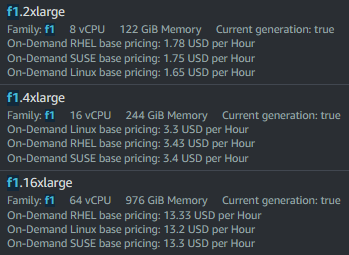
\includegraphics[width=.6\textwidth]{img/f1_costs.png}
        \end{figure}
    \end{enumerate}

    \longline

    \subsubsection{Some interesting blog posts \& articles}

    \begin{itemize}
        \item \href{https://aws.amazon.com/blogs/publicsector/university-of-berkeley-uses-aws-educate-for-amazon-fpga-accelerator-development-and-deployment-in-the-cloud/}{University of California, Berkeley uses AWS Educate and Amazon FPGA Instances in Undergraduate Computer Architecture Course} by AWS Public Sector Blog Team

        \item \href{https://aws.amazon.com/blogs/startups/competition-forever-change-blockchain/}{Time, Randomness, and a \$100,000 Prize to Forever Change Blockchain} by Michael V. Copeland

        \item \href{https://aws.amazon.com/blogs/apn/how-dnanexus-and-edico-genome-are-powering-precision-medicine-on-amazon-web-services-aws/}{How DNAnexus and Edico Genome are Powering Precision Medicine on Amazon Web Services (AWS)} by Aaron Friedman and Ujjwal Ratan

        \item \href{https://aws.amazon.com/blogs/compute/bringing-datacenter-scale-hardware-software-co-design-to-the-cloud-with-firesim-and-amazon-ec2-f1-instances/}{Bringing Datacenter-Scale Hardware-Software Co-design to the Cloud with FireSim and Amazon EC2 F1 Instances} by Mia Champion

        \item \href{https://aws.amazon.com/blogs/compute/accelerating-precision-medicine-at-scale/}{Accelerating Precision Medicine at Scale} by Aaron Friedman and Angel Pizarro
    \end{itemize}

    \newpage

    \section{Microsoft}

    \subsection{Azure Stack Edge Pro FPGA (Expired on February 2024)}

    Microsoft provided an interesting service called \href{https://learn.microsoft.com/en-us/azure/databox-online/azure-stack-edge-overview}{Azure Stack Edge Pro FPGA}. In summary, it's an AI-enabled edge computing device with network data transfer capabilities. Unfortunately, these interesting devices will reach end-of-life in February 2024. If you are considering new deployments, Microsoft recommend that you explore Azure Stack Edge Pro 2 (section \ref{subsection: azure stack edge pro 2} page \pageref{subsection: azure stack edge pro 2}) or Azure Stack Edge Pro GPU (\href{https://learn.microsoft.com/en-us/azure/databox-online/azure-stack-edge-gpu-overview}{Azure Stack Edge Pro with GPU}) devices for your workloads.\newline

    \noindent
    Azure Stack Edge Pro with FPGA is a Hardware-as-a-service solution. Microsoft ships you a cloud-managed device with a built-in Field Programmable Gate Array (FPGA) that enables accelerated AI-inferencing and has all the capabilities of a network storage gateway.\newline

    \noindent
    Azure Data Box Edge is rebranded as Azure Stack Edge. You can find it in the marketplace on Azure Cloud Platform. Again, this product will expired, so you can order only Pro 2 or Pro GPU.\newline

    \noindent
    In the following pages you can find the researches making to find what Microsoft offers. An interesting official documentation is available online at \href{https://learn.microsoft.com/en-us/azure/databox-online/azure-stack-edge-overview}{this link} or you can read the offline documentation findable in \texttt{resources} path in this project (\href{https://github.com/AndreVale69/FPGA-project-presentation/blob/main/resources/Azure%20Stack%20Edge%20-%20Documentation.zip}{or online in my GitHub repository}).

    \begin{figure}[!htp]
        \centering
        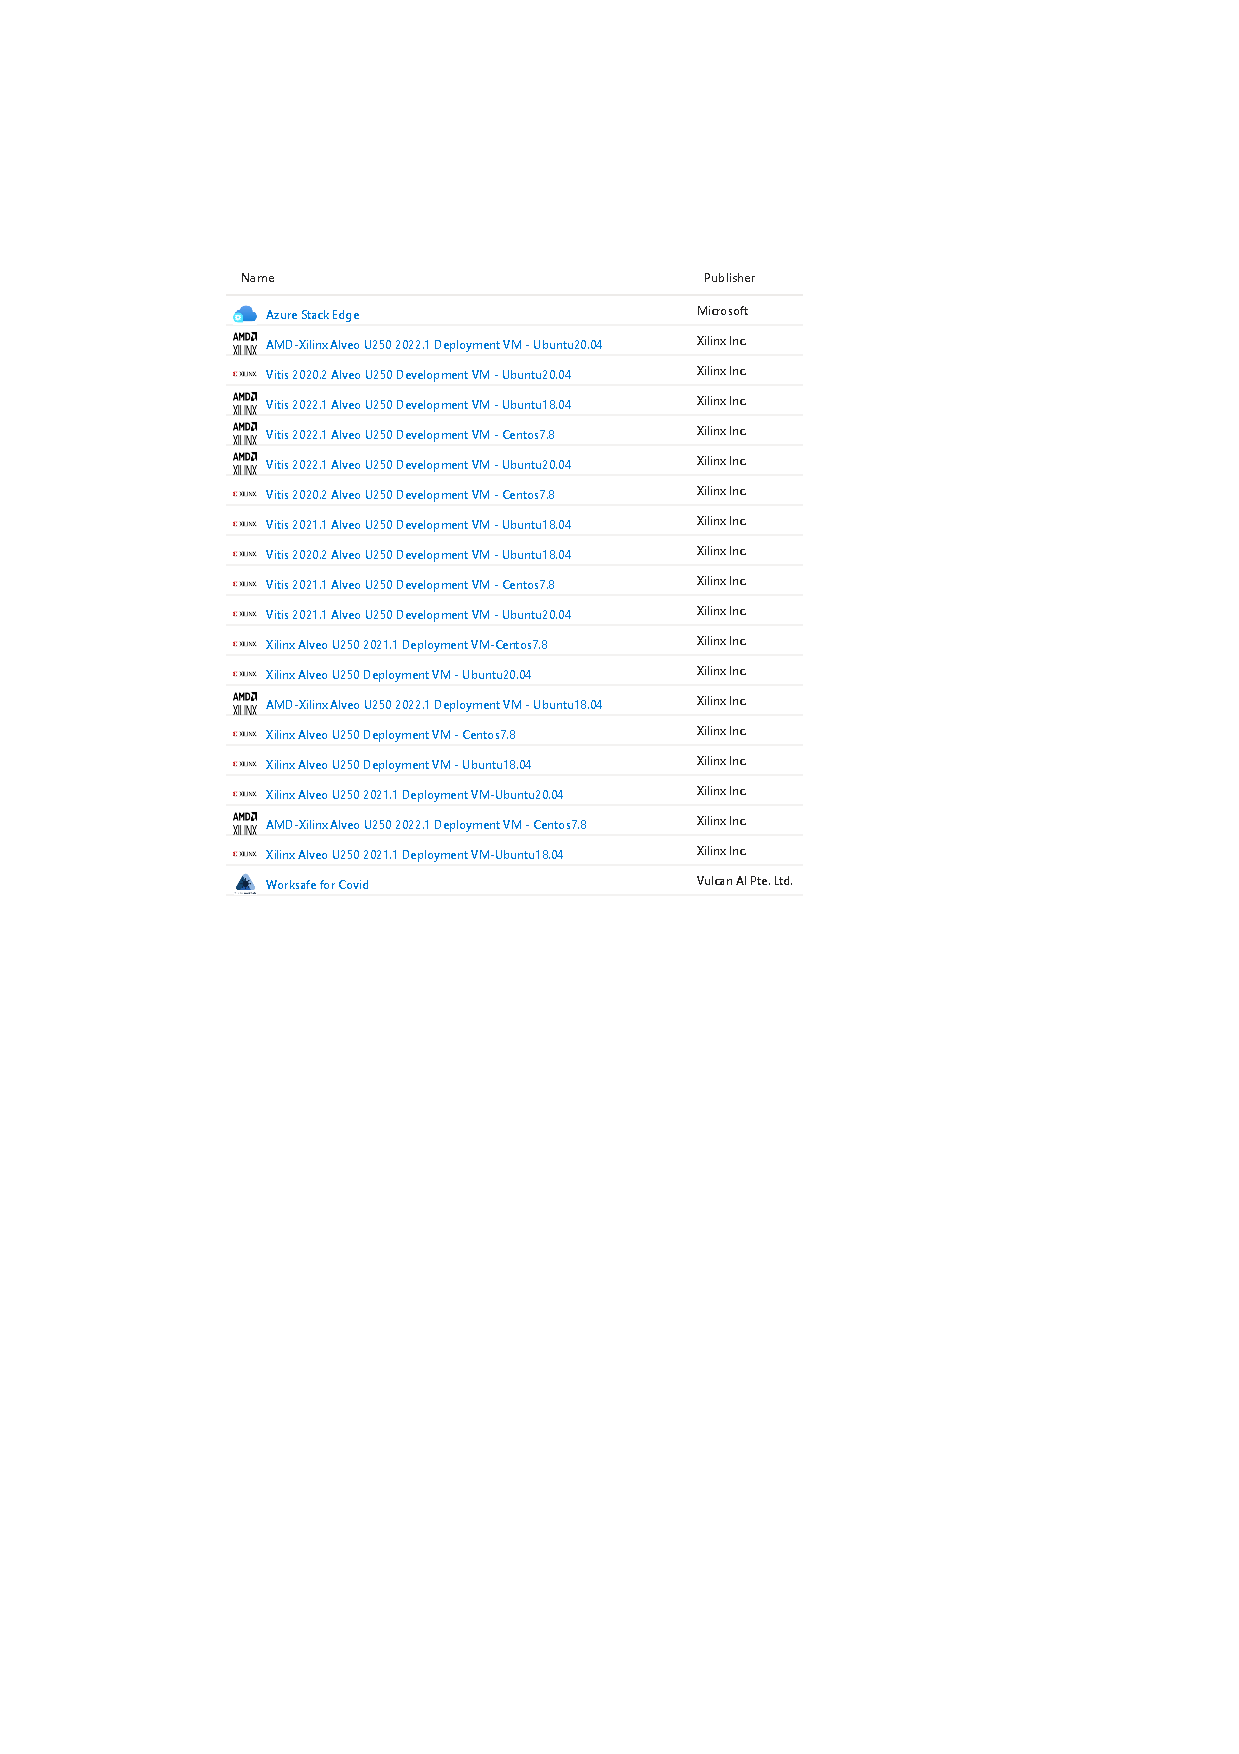
\includegraphics[width=\textwidth]{img/Marketplace FPGA - Microsoft Azure.pdf}
        \caption{Using a student account on Microsoft Azure, you can search what do you want on Marketplace. It's also \href{https://azuremarketplace.microsoft.com/en/marketplace/apps?search=fpga&page=1}{available online}. The services provided by AMD are Virtual Machines. In this devices you can find softwares to develop FPGA. Despite, \href{https://azuremarketplace.microsoft.com/en/marketplace/apps/Microsoft.DataBoxEdge?tab=Overview}{Azure Stack Edge} is used for over-the-network high performance data transfers. Azure Stack Edge physical devices are available in various form factors and can be tailored for harsh environmental conditions.}
    \end{figure}

    \newpage

    \subsection{Azure Stack Edge Pro 2}\label{subsection: azure stack edge pro 2}

    \href{https://learn.microsoft.com/en-us/azure/databox-online/azure-stack-edge-pro-2-overviewURL}{Azure Stack Edge Pro 2} is an evolution of Azure Stack Edge. It uses one or two GPU and is often used for rapid Machine Learning (ML) inferencing.\newline

    \noindent
    \emph{Azure Stack Edge Pro 2} is a new generation of an \textbf{AI-enabled edge computing device} offered as a service from Microsoft. It offers the following benefits over its precursor, the Azure Stack Edge Pro series:
    \begin{itemize}
        \item This series offers multiple models that closely align with your compute, storage, and memory needs. Depending on the model you choose, the compute acceleration could be via one or two Graphical Processing Units (GPU) on the device.
        
        \item This series has flexible form factors with multiple mounting options. These devices can be rack mounted, mounted on a wall, or even placed on a shelf in your office.
        
        \item These devices have low acoustic emissions and meet the requirements for noise levels in an office environment.
    \end{itemize}
    \begin{flushleft}
        \textbf{\underline{Use cases}}
    \end{flushleft}
    The Pro 2 series is designed for deployment in edge locations such as retail, telecommunications, manufacturing, or even healthcare. Here are the various scenarios where Azure Stack Edge Pro 2 can be used for rapid Machine Learning (ML) inferencing at the edge and preprocessing data before sending it to Azure.
    \begin{itemize}
        \item \textbf{Inference with Azure Machine Learning} - With this solution, you can run ML models to get quick results that can be acted on before the data is sent to the cloud. The full data set can optionally be transferred to continue to retrain and improve your ML models. For more information, see how to \href{https://learn.microsoft.com/en-us/azure/machine-learning/how-to-deploy-fpga-web-service#deploy-to-a-local-edge-server}{Deploy Azure ML hardware accelerated models on Azure Stack Edge}.

        \item \textbf{Preprocess data} - Transform data before sending it to Azure via compute options such as containerized workloads and Virtual Machines to create a more actionable dataset. Preprocessing can be used to:
        \begin{itemize}
            \item Aggregate data.
            \item Modify data, for example, to remove personal data.
            \item Subset data to optimize storage and bandwidth, or for further analysis.
            \item Analyze and react to IoT Events.
        \end{itemize}

        \item \textbf{Transfer data over network to Azure} - Use this solution to easily and quickly transfer data to Azure to enable further compute and analytics or for archival purposes.
    \end{itemize}

    \newpage

    \subsection{Azure Stack Edge Pricing}\label{subsection: azure stack edge pricing}

    The devices seen in the previous chapters, can be ordered from the \href{https://learn.microsoft.com/en-us/azure/azure-edge-hardware-center/azure-edge-hardware-center-overview}{Azure Edge Hardware center}. These devices are billed as a monthly service through the Azure portal. For more information, see \href{https://azure.microsoft.com/en-gb/pricing/details/azure-stack/edge/#pricing}{pricing}.

    \begin{table}[!htp]
        \centering
        \begin{tabular}{@{} l p{10em} l @{}}
            \toprule
            \textbf{Service} & \textbf{Unit} & \textbf{Price} \\
            \midrule
            Monthly subscription fee & 1 unit with GPU & \textbf{\geneuro646} \\
            \\
            %
            Monthly subscription fee & 1 unit with 2 GPUs & \textbf{\geneuro811} \\
            \\
            %
            Monthly subscription fee & 1 unit with FPGA & Expired \\
            \\
            %
            Shipping - US & 1 unit & \textbf{\geneuro316} \\ \\
            Shipping - EMEA & 1 unit & \textbf{\geneuro316} \\ \\
            Shipping - APAC & 1 unit & \textbf{\geneuro316} \\ \\
            Shipping - Americas & 1 unit & \textbf{\geneuro316} \\
            \bottomrule
        \end{tabular}
        \caption{\href{https://learn.microsoft.com/en-us/azure/databox-online/azure-stack-edge-overview}{Azure Stack Edge Pro FPGA}}
    \end{table}
    \begin{table}[!htp]
        \begin{tabular}{@{} l p{18em} l @{}}
            \toprule
            \textbf{Service} & \textbf{Unit} & \textbf{Price} \\
            \midrule
            Monthly subscription fee & Model: 64G2T\newline 32 vCPUs, 51 GB RAM, 720 GB & \textbf{\geneuro359} \\
            \\
            %
            Monthly subscription fee & Model: 128G4T1GPU\newline 32 vCPUs, 102 GB RAM, 1.6 TB, 1 x NVIDIA A2 GPU & \textbf{\geneuro469} \\
            \\
            %
            Monthly subscription fee & Model: 256G6T2GPU\newline 32 vCPUs, 204 GB RAM, 2.5 TB, 2 x NVIDIA A2 GPUs & \textbf{\geneuro554} \\
            \\
            %
            Shipping & 1 unit & \textbf{\geneuro316} \\
            \bottomrule
        \end{tabular}
        \caption{\href{https://learn.microsoft.com/en-us/azure/databox-online/azure-stack-edge-pro-2-overviewURL}{Azure Stack Edge Pro 2}}
    \end{table}

    \newpage

    \section{Intel}\label{section: Intel}

    \subsection{Developer Clouds for Accelerated Computing}

    \href{https://www.intel.com/content/www/us/en/developer/tools/devcloud/overview.html}{Developer Clouds for Accelerated Computing} is an online platform used to learn, prototype, test and run applications and workloads on a cluster of the latest Intel hardware and software.\newline

    \noindent
    It offers several configurations that are tuned to various workloads. From AI and inference training to FPGA development to edge prototyping and preproduction deployment, you can use the environment that best matches your business needs.
    \begin{itemize}
        \item Learn with hands-on tutorials.
        \item Experiment with real-world code samples.
        \item Evaluate performance and acceleration with multiple hardware configurations.
        \item Build heterogeneous applications.
        \item Develop your own prototype.
        \item Benchmark your own AI workloads with always-on access to the latest AI hardware.
    \end{itemize}
    Available Intel Hardware:\newline

    \noindent
    \begin{minipage}{.18\textwidth}
        
\includegraphics[width=\textwidth]{img/xeon_logo.png}
    \end{minipage}
    \begin{minipage}{.18\textwidth}
        
\includegraphics[width=\textwidth]{img/xeon_max_series_logo.png}
    \end{minipage}
    \begin{minipage}{.18\textwidth}
        
\includegraphics[width=\textwidth]{img/data_center_gpu_flex_series_logo.png}
    \end{minipage}
    \begin{minipage}{.18\textwidth}
        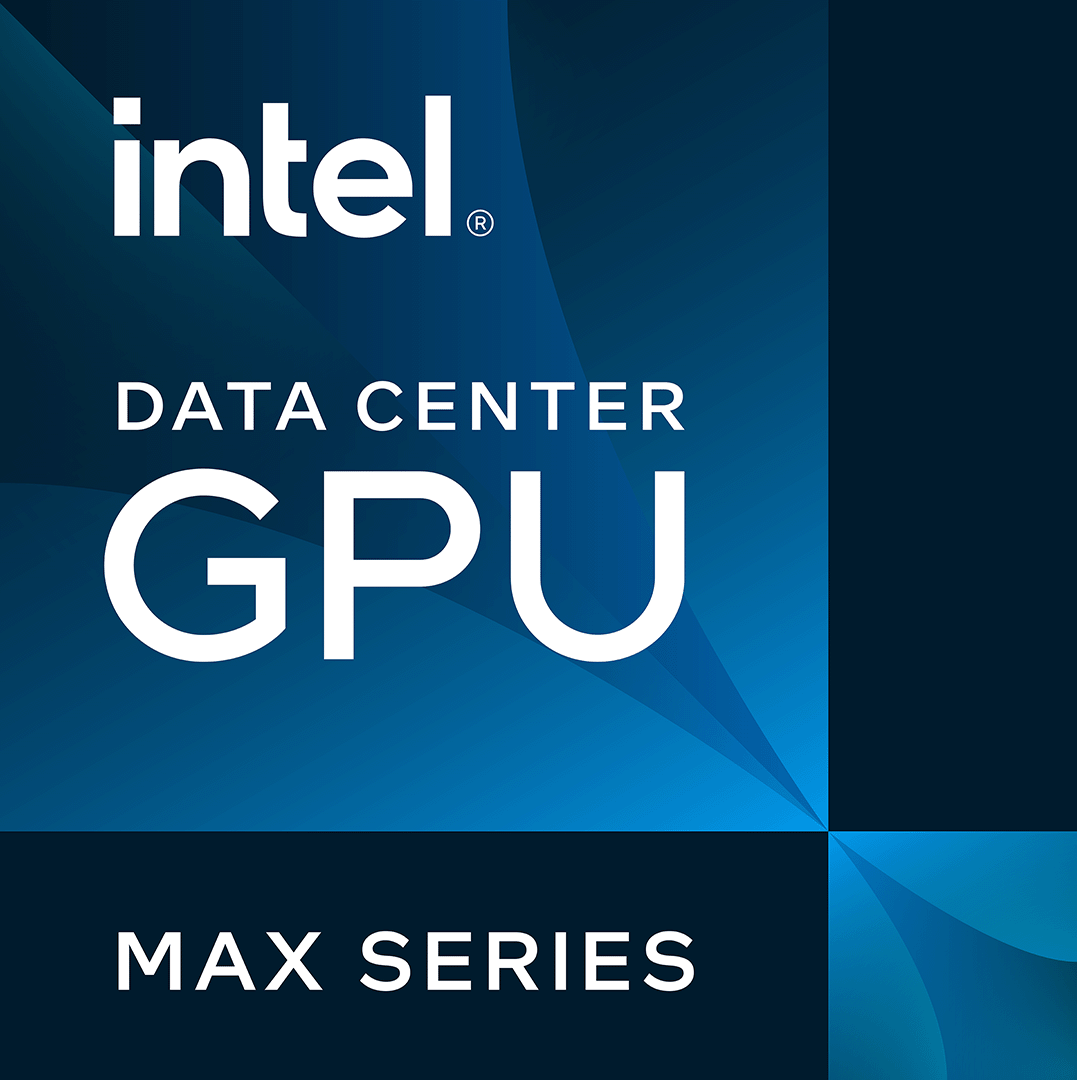
\includegraphics[width=\textwidth]{img/data_center_gpu_max_series_logo.png}
    \end{minipage}
    \begin{minipage}{.18\textwidth}
        
\includegraphics[width=\textwidth]{img/gaudi_logo.png}
    \end{minipage}

    \begin{itemize}
        \item \href{https://www.intel.com/content/www/us/en/products/details/processors/xeon.html}{Intel Xeon Processors}
        \item \href{https://www.intel.com/content/www/us/en/products/details/discrete-gpus/data-center-gpu.html}{Intel Data Center GPU}
        \item \href{https://www.intel.com/content/www/us/en/developer/articles/technical/habana-gaudi2-processor-for-deep-learning.html}{Gaudi 2} and Gaudi 3 (not yet released, \href{https://www.intel.com/content/www/us/en/newsroom/news/ai-everywhere-core-ultra-5th-gen-xeon-news.html}{official sneak peek})
    \end{itemize}\newpage

    \subsection{Build Multiarchitecture and FPGA Applications}

    Intel allows you to test performance on CPU, GPU and FPGA architectures. But to do this, you need to log in to their platform \href{https://devcloud.intel.com/oneapi/home/}{Build Multiarchitecture and FPGA Applications}. Here you can get some information such as featured tools, frameworks and libraries, an exhaustive \href{https://devcloud.intel.com/oneapi/documentation/shell-commands/}{documentation} and a \href{https://devcloud.intel.com/oneapi/get_started/}{list of their products} given once you have done the registration.

    \begin{figure}[!htp]
        \centering
        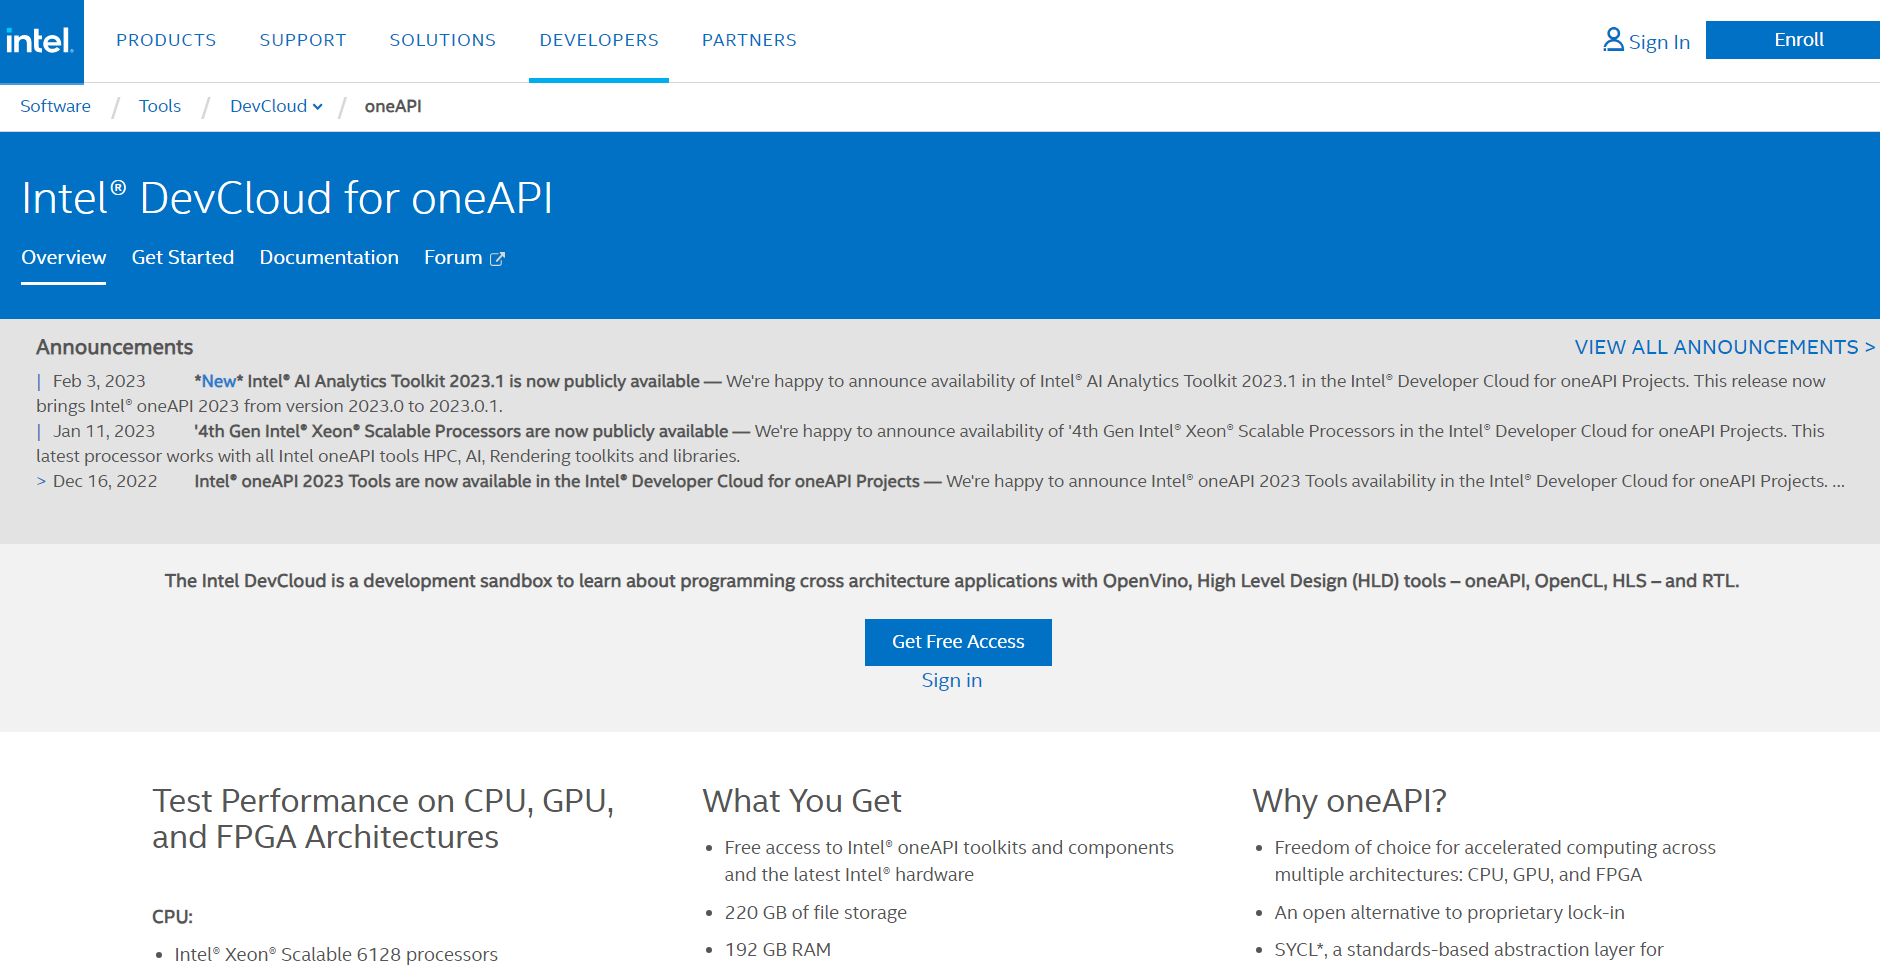
\includegraphics[width=\textwidth]{img/Intel_DevCloud_for_oneAPI.png}
        \caption{\href{https://devcloud.intel.com/oneapi/home/}{Build Multiarchitecture and FPGA Applications} (click \href{https://github.com/AndreVale69/FPGA-project-presentation/tree/main/document/ENG-version/img/Intel_DevCloud_for_oneAPI.png}{here} to see the image full screen)}
    \end{figure}

    \noindent
    The following list only covers the toolkits used for FPGA purposes:
    \begin{itemize}
        \item \textbf{OpenCL for FPGA development}. Intel FPGA SDK for OpenCL software technology is a development environment that enables software developers to accelerate their applications by targeting heterogeneous platforms with Intel CPUs and FPGAs.
        
        Features offered:
        \begin{itemize}
            \item Microsoft Visual Studio or Eclipse-based Intel Code Builder for\newline OpenCL API now with FPGA support;

            \item Fast FPGA emulation based on Intel's compiler technology;

            \item Create OpenCL project jump-start wizard;
            
            \item Development Environment for both host (CPU) and accelerator\newline (FPGA);

            \item Syntax highlighting and code auto-completion features;
            
            \item FPGA resource and performance analysis;
            
            \item Fast and incremental FPGA compile.
        \end{itemize}
        This is the link to the \href{https://github.com/intel/FPGA-Devcloud/tree/master/main/QuickStartGuides/OpenCL_Program_PAC_Quickstart}{GitHub repository} to get started with a first sample.

        \item \textbf{RTL Acceleration Functional Unit}. The Intel Quartus Prime Design Software includes everything you need to design for Intel FPGAs, SoCs, and complex programmable logic device (CPLD) from design entry and synthesis to optimization, verification, and simulation. Dramatically increased capabilities on devices with multi-million logic elements are providing designers with the ideal platform to meet next-generation design opportunities.

        Build and design using standard logic gates. Great for visualization and education.

        This the link to the \href{https://github.com/intel/FPGA-Devcloud/tree/master/main/QuickStartGuides/RTL_AFU_Program_PAC_Quickstart}{GitHub repository} to get started with a first sample.
    \end{itemize}

    \longline

    \subsubsection{Create an account}

    To create an account click on the \href{https://www.intel.com/content/www/us/en/secure/forms/devcloud/enrollment.html}{\emph{Get Free Access}} button. This will take you to a login/register page. You can also enter a personal email here, as Intel's services don't check this (I can't find any resources that say a personal email is not allowed).

    Once you have entered your email and password, and confirmed the email with a code, Intel will ask you a few questions when you log in:
    \begin{itemize}
        \item Information about yourself:
        \begin{itemize}
            \item Business or Institution Name.
            \item What type of user are you? The possibility are: researcher, student, teacher/professor, etc.
        \end{itemize}

        \item Read and accept Intel Developer Cloud Terms and Conditions (available offline in \texttt{resources} path or \href{https://github.com/AndreVale69/FPGA-project-presentation/tree/main/resources/Intel%20Developer%20Cloud%20-%20Terms%20and%20Conditions.pdf}{online at my GitHub repository})
    \end{itemize}
\end{document}